\chapter{File formats}\label{annex:file-formats}

\section{ASCII fishing data files}\label{appendix-ascii}

\subsection{Effort and catch}\label{sec:EC-datafile}

The raw geo-referenced effort and catch data is a voluminous dataset containing the information on fishery, gear, date, lon-lat coordinates, spatial resolution as well as corresponding records of effort and catch. In order to be correctly interpreted by the SEAPODYM software, the data should be organised and formatted as described below. Note that it is advised to keep the original spatial resolution of fisheries data. This avoids unnecessary inflation of the ASCII file and allows fitting the catch at original spatial resolution. As described in Chapter~\ref{ch:parametrisation} (section~\ref{sec:predicted-catch}), the uniform distribution of fishing effort or catch is implemented in the code in order to ensure that the fishing mortality is always applied at the spatial resolution of the model.       
  
The effort and catch data file format is shown below. It is a tabulation-separated ASCII file with extension .txt, having a small header followed by the table with row names as follows (example):

\vspace{1cm}
{\ttfamily
  \noindent \hspace*{0.5cm} 7} 
 \hspace*{9.25cm}  \textit{{\color{blue}$\leftarrow$ number of fisheries}}\\
{\ttfamily  \hspace*{0.5cm} 84286 52530 47545 21675 3354 158510  120459} 
 \hspace*{0.5cm}\textit{{\color{blue}$\leftarrow$ number of records by fishery}}\\
{\ttfamily  \hspace*{0.5cm} f yr \mbox{ } mm dd gr lat lon \mbox{ } res E  \mbox{ } C}
 \hspace*{2cm}\textit{{\color{blue}$\leftarrow$ column names}}\\
{\ttfamily  \hspace*{0.5cm} 1 1950 8 \text{ }15 L \mbox{} 7.5 152.5 5 \mbox{ } 60 \mbox{ }1.118}
 \hspace*{1.15cm}\textit{{\color{blue}$\leftarrow$ the first record in the file}}\\
  \hspace*{0.65cm} $\dots$
\vspace{0.5cm}		

The detailed description of each record is provided in Table~\ref{tab:EC-fformat}.  Note, the name of the fishery is read by the code as the concatenation of letter in {\ttfamily gr} and the ID in {\ttfamily f}. For example, the record above belongs to fishery 'L1'. Hence, each unique combination of gear and ID is interpreted as a stand-alone fishery and the number of fisheries as well as number of records for each fishery must correspond to the information provided in the header. Consequently, all fisheries present in this file have to be defined in the configuration parfile in order to be taken into account.   

\vspace*{2cm}
\begin{table}
\caption{The information written in the input geo-referenced effort and catch data file prepared for the SEAPODYM software.}
  \vspace{0.25cm}
\begin{tabular}{p{1.65cm}p{12.0cm}p{1.75cm}}
    \hline
   {\bfseries Column name} & {\bfseries Description} & {\bfseries Type}\\ \hline\hline
   {\ttfamily f} & Fishery ID & integer\\  \hline
   {\ttfamily yr} & Year of catch & integer\\ \hline
   {\ttfamily mm} & Month of catch & integer\\ \hline
   {\ttfamily dd} & Day of catch  & integer\\ \hline
   {\ttfamily gr} & Usually a single letter denoting fishing gear. Examples: L for longline, S for purse-seine, P for pole and line, T for troll, O for other (combination of different gears) & character\\ \hline
   {\ttfamily lat} & Latitudinal coordinate of the centre of the square, in which the catch data was aggregated, given in digital degrees & float\\ \hline
   {\ttfamily lon} & Longitudinal coordinate of the centre of the square, in which the catch data was aggregated, given in digital degrees & float\\ \hline
   {\ttfamily res} & The size of the square in which the catch data was aggregated, in degrees; should be unique by fishery & float \\ \hline
    {\ttfamily E} & Fishing effort, can be given in different units; the units are implicit (affect the catchability coefficients) and should be unique within a given fishery & float   \\ \hline
    {\ttfamily C} & Catch of a given species; the units, usually metric tonnes or number of individuals, are not stored in this file and should be unique through all fisheries in the file & float\\ \hline
\end{tabular}
\label{tab:EC-fformat}
\end{table}

\subsection{Size frequencies}\label{sec:LF-datafile}
Although it is strongly recommended to use the length frequency (LF) data in SEAPODYM to facilitate parameter estimation, it is possible to run SEAPODYM without size frequency data by setting flag {\ttfamily frq\_likelihood} and number of LF files {\ttfamily file\_frq\_data} to 0. Since the LF data are provided at coarse spatio-temporal resolution, usually over quarter and rectangular region, and because the data are size structured, the file format is very different from effort and catch data file. However, the same fisheries, partially or entirely, must be present in the LF file. Besides, the region of LF record must contain at least one record with effort and catch data to be taken into account. 

Several LF files can be provided as the SEAPODYM input. The splitting is necessary once the size structure of the data is not homogeneous. For example, the catch at size provided for at 2~cm bins cannot be combined with the data at 1~cm bins. Each LF file consists of the header with regional structure of the LF data and the table, which contains the information on date, region, fishery and the catch at size records. The LF file is the tabulation-separated ASCII  file with extension .txt having the following structure (example):

\vspace{1cm}
{\ttfamily \noindent
  \hspace*{0.5cm} 668 \mbox{} 7 \mbox{} 20809}
 \hspace*{1.1cm}  \textit{{\color{blue}$\leftarrow$ nb. of unique regions \mbox{ } nb. of fisheries \mbox{ } total nb. of records}}\\
{\ttfamily  \hspace*{0.5cm} 1	110 115     15      20 }
 \hspace*{0.5cm}  \textit{{\color{blue}$\leftarrow$ region ID \mbox { } regional coordinates}}\\  
{\ttfamily  \hspace*{0.5cm} $\dots$}
\hspace*{3.4cm}  \textit{{\color{blue}$\leftarrow$ all other regions from 2 to 668}}\\
{\ttfamily  \hspace*{0.5cm} 11      20      5}
 \hspace*{2.5cm}  \textit{{\color{blue}$\leftarrow$ number of bins \mbox{ } first bin size \mbox{ } bin size}}\\    
{\ttfamily  \hspace*{0.5cm} yr      qtr     mo      f       reg     LF[1] .. LF[11]}
 \hspace*{1.5cm}  \textit{{\color{blue}$\leftarrow$ column names of the main table}}\\  
{\ttfamily  \hspace*{0.5cm} 1955    1       1       L1      2       0       0      0       0       5            37      19      18      4       1       0  }
 \hspace*{0.0cm}  \textit{{\color{blue}$\leftarrow$ standard LF record}}\\  
{\ttfamily  \hspace*{0.5cm} $\dots$ }\\

\noindent where regional coordinates should be written as tab-separated (lon-west, lon-east, lat-south, lat-north) set. The detailed description of the LF record is provided in Table~\ref{tab:LF-fformat}. Note that since the LF data are usually quarterly, column 'month' is redundant and contains the first month of quarter, however it can potentially be used in case if higher resolution data will be available. 

\begin{table}[H]
\caption{Structure of {\ttfamily length frequencies} data file.}
  \vspace{0.5cm}
\begin{tabular}{p{1.65cm}p{12.0cm}p{1.75cm}}
    \hline
   {\bfseries Column name} & {\bfseries Description} & {\bfseries Type}\\ \hline\hline
    {\ttfamily yr}& The year of the LF sample & integer \\ \hline
    {\ttfamily qtr}& The quarter of the LF sample & integer \\ \hline
    {\ttfamily mo}& The month of the LF sample or the first month of the quarter for seasonal data & integer \\ \hline    
    {\ttfamily f}& Here the fishery name as in the effort and catch file and in the parfile & character \\ \hline
    {\ttfamily reg} & The ID of the region of a given sample & integer\\ \hline
    {\ttfamily LF[i]} & The number of fish caught in the size bin $i$, this number can be raised to total catch & float  \\ \hline
\end{tabular}
\label{tab:LF-fformat}
\end{table}

\section{ASCII output files}\label{annex:text-files}

\subsection{SumDym.txt}\label{annex:sumdym}

All ASCII output files in SEAPODYM are tabulation-separated. The SumDym.txt file contains the time evolution of the model variables aggregated over the model domain, i.e. for each variable $\phi(x,y,t)$ either used as model forcing or computed by the model it has $\sum\limits_{x,y}\phi(x,y,t)$. The scheme in Figure~\ref{fig:variables-sumdym}~\ illustrates the structure of this file. The data are written in tabular form. The one-line header contains the names of the table columns. The dimension, i.e. number of columns and rows in this file depends on the current run configuration specified in the parfile, with the number of rows being the number of time steps $n_{t}$, and number of columns depending on number of life stages and number of fisheries. 

\begin{table}
\begin{center}
\begin{tabular}{c}
$
\overbrace{2}^{\text{date, tstep}}+ \underbrace{3}_{\text{Primary production in C-C}} + \overbrace{1}^{\text{Sum over P in C-C}}+\underbrace{n_{forage}}_{\text{\makecell{Biomass of each\\ functionnal group.}}}+$ \\
$\overbrace{n_{life\mbox{ }stage}}^{\text{\makecell{Biomass\\ per life stage\\spname}}}+\underbrace{1}_{\text{\makecell{Total biomass of\\spname }}}+\overbrace{n_{f}\times 5}^{\text{\makecell{Fishing effort, observed and predicted catch\\ Observed and predicted CPUE, by fishery}}} 
$
\end{tabular}
\end{center}
\captionof{figure}{The structure of SumDym.txt file. The coordinates $C-C$ correspond to three regional aggregations of the primary production $P$: 10$^\circ$N-45$^\circ$N, 10$^\circ$S-10$^\circ$N and 35$^\circ$S-10$^\circ$S, where longitudinal extension corresponds to that of model domain. The number of columns $n_{forage}$, $n_{life\mbox{ }stage}$, $n_{f}$ denote the number of micronekton groups, the number of life stages and the number of fisheries respectively. } 
\label{fig:variables-sumdym}
\end{table}


\subsection{SumQArea.txt}\label{annex:sumqarea}

This file is similar to SumDym.txt, however instead of aggregation over the model domain, it contains model variables aggregated over regional structure defined in the parfile (see section~\ref{sec:aggregation} for more details). Also, this file does not contain fisheries stattistics. The file header provides essential details on regional structure defined in the current run and the definition of life stages. Thus, first $n_{reg}$ lines are filled with regional coordinates corresponding to the corners of rectangular regions, written as follows: westmost longitude, eastmost longitude,  southern latitude, northern latitude. Regions are followed by the summary of the species life stages among larvae, juvenile, young and adult as well as the indices of age classes included within each life stage. Note, since this file is mostly used for comparisons with regional stock assessment estimates, recruits are also written, although it is not a life stage in SEAPODYM, but simply an age class that corresponds to the definition of recruitment to the exploited population used in the stock assessment model.

The main table has the header denoting column names. The number of rows of this table corresponds to the number of model time steps, $n_{t}$, and columns as shown schematically in Figure~\ref{fig:variables-sumqarea}.

\begin{table}
\begin{center}
\begin{tabular}{c}
$
\underbrace{3}_{\text{year\mbox{ }month\mbox{ }day}}+\overbrace{n_{reg}}^{\text{\makecell{Nb. of larvae \\ per region}}}+\underbrace{1}_{\text{\makecell{Nb. of larvae \\ over all regions}}}+\overbrace{n_{reg}}^{\text{\makecell{Nb. of small juveniles  \\ per region}}}+\underbrace{1}_{\text{\makecell{Nb. of small juveniles \\ over all regions}}}$\\
$+\overbrace{n_{reg}}^{\text{\makecell{Biomass at young stage\\ per region}}}+\underbrace{1}_{\text{\makecell{Biomass at young stage \\ over all regions}}}+\overbrace{n_{reg}}^{\text{\makecell{Biomass at adult stage  \\ per region}}}+\underbrace{1}_{\text{\makecell{Biomass at adult stage \\ over all regions}}}$\\
$+\overbrace{n_{reg}}^{\text{\makecell{Biomass at young and adult stages\\ per region}}}+\underbrace{1}_{\text{\makecell{Total biomass at young and adult stages \\ over all regions}}}$
\end{tabular}
\captionof{figure}{The structure of {\ttfamily SumQArea.txt} file. }
\label{fig:variables-sumqarea}
\end{center}
\end{table} 


\subsection{SumEEZ.txt}\label{annex:sumeez}

The tabulation-separated file {ttfamily SumEEZ\_EEZname.txt} contains the time evolution of biomass extractions over selected EEZ area. The structure of this file is shown in Figure~\ref{fig:variables-sumeez}. The number of columns is fixed, and the aggregated statistics is computed for larvae, small juveniles, recruits (same definition as for SumQArea.txt) young (immature adults) and mature adults. The last column contains the sum of biomass at young and adult life stages. 

\begin{table}
\begin{center}
\begin{tabular}{c}
$\underbrace{3}_{\text{year\mbox{ }month\mbox{ }day}}+\overbrace{3}^{\text{\makecell{Nb. of larvae, small juveniles \\ and recruits in EEZ}}}+\underbrace{2}_{\text{\makecell{Biomass at young \\ and adult stage}}}+\overbrace{1}^{\text{\makecell{Total biomass\\ sum of young and adult}}}$\\
\end{tabular}
\captionof{figure}{The structure of {\ttfamily SumEEZ.txt} file. }
\label{fig:variables-sumeez}
\end{center} 
\end{table}


\subsection{MeanVar.txt}\label{annex:meanvar}

This ASCII output file {\ttfamily spname\_MeanVar.txt} is used to analyse the temporal evolution of aggregated model variables at age, with the aggregation method being the weighted mean and weights being the spatial distribution of population density. The aggregated variables are: 1) natural mortality at age, 2) species speed at age, 3) species diffusion rate at age, and 4) the ambient water temperature at age. The information is structured into a matrix of $n_{t}$ rows and the number of columns depending on the number of age classes. See Figure~\ref{fig:variables-meanvar} for more details.
 
\begin{table} [H]
\begin{center}
\begin{tabular}{c}
$
\underbrace{3}_{\text{year-month-day}}+\overbrace{n_{a}\times 4}^{\text{\makecell{Weighted mean of model variables at age $a$ \footnotemark[1]}}}
$
\end{tabular}
\captionof{figure}{The structure of {\ttfamily spname\_MeanVar.txt} file. }
\label{fig:variables-meanvar}
\end{center}
\end{table}

\footnotetext[1]{with $a$ varying from $0$ to the maximum age $A^{+}$ defined in the model run.}

\subsection{Spatial\_Corr.txt}\label{annex:spcorr}
The ASCII file {\ttfamily spname\_Spatial\_Corr.txt} contains correlation statistics for catch and CPUE data. The number of rows in this file is equal to the number of time steps $n_{t}$, and the columns, reading from the left to right of the matrix, are structured as shown in Figure~\ref{fig:variables-spcorr} :

\begin{table} [H]
\begin{center}
\begin{tabular}{c}
$
\underbrace{1}_{\text{date}}+\underbrace{n_{ij}+r(C^{obs}_f,C^{pred}_f)+p_C+r(CPUE^{obs}_f,CPUE^{pred}_f)+p_{CPUE}}_{n_f}
$\\
\end{tabular}
\captionof{figure}{The structure of {\ttfamily spname\_Spatial\_Corr.txt} file. The date is written as 'YYYY-mm'. The number $n_{ij}$ is the number of spatial observations for a given fishery $f$ and time step.}
\label{fig:variables-spcorr}
\end{center}
\end{table}

The $C$-code that computes the correlation is based on a script detailed in the book \textit{'Numerical Recipes in C, Press and al. 1994 (14.5 p. 638)}. 
If we denote $X$ the observed variable, and $Y$ the estimated one, then at each time step we the spatial correlations are computed as follows:

\begin{align*}
\delta_X\left(i,j\right) &= X\left(i,j\right)-\left< X\left(i,j\right)\right>_{i,j} \\
C_{XY} &= \left<\delta_X\delta_Y\right>_{i,j} \\
r &= \frac{C_{XY}}{\sqrt{C_{XX}C_{YY}}} \\
\end{align*}

\subsection{LF\_obs.txt}\label{annex:lfobs}
File {\ttfamily spname\_LF\_obs.txt} stores the observed quarterly and annual length frequency data read by SEAPODYM redistributed to the model age structure and aggregated by fishery and region. Note, if the regional structure is not activated in the parfile, that is {\ttfamily nb\_region\_sp\_B = 0} in the aggregation section, then the regional structure of the LF data is used to write this file, leading to usually a very big file size. 

Since both age and regional information is written over quarters, the file contains five table, corresponding to four quarterly and one annual aggregation of the catch-at-age data. The number of rows in each table is equal to the number of age classes and the number of columns depends on the number of fisheries and regions in the model configuration. Each line in these tables is structured as shown in Figure~\ref{fig:variables-lfobs}: 

\begin{table}[H]
\begin{center}
\begin{tabular}{c}
$
\underbrace{1}_{\text{length-at-age}}+\overbrace{n_f}^{\text{\makecell{Catch-at-age by fishery \\in region 1}}}  \cdots  \overbrace{n_f}^{\text{\makecell{Catch-at-age by fishery \\in region $n_{reg}$}}} + \underbrace{n_f}_{\text{\makecell{Total catch-at-age \\ by fishery over all regions}}} + \overbrace{n_{reg}}^{\text{\makecell{Total catch-at-age \\ by region}}}
$
\end{tabular}
\captionof{figure}{The structure of quarterly or annual LF data in {\ttfamily spname\_LF\_obs.txt} file. The mean length-at-age is written in cm.}
\label{fig:variables-lfobs}
\end{center}
\end{table}

 
\subsection{LF\_Q\_fishery.txt}\label{sec:lfqfishery}

The data structure in file {\ttfamily spname\_LF\_Q\_fishery.txt} is similar to that in the input file {\ttfamily spname\_LF.txt} described in section~\ref{sec:LF-datafile}. The difference with the input data file is that here the LF data are aggregated to the model age classes. The file header is written as follows (example of the skipjack model configuration):

\vspace{0.5cm}
{\ttfamily \noindent
  \hspace*{0.5cm} 5 \mbox{  } 15}
  \hspace*{5cm}  \textit{{\color{blue}$\leftarrow$ number of regions \mbox{} number of fisheries}}\\
  \hspace*{0.5cm} 11.65   16.91   21.83   26.43 $\dots$
  \hspace*{1.5cm}  \textit{{\color{blue}$\leftarrow \ell_{J+1} \mbox{ } \ell_1 \mbox{ } \dots \mbox{ } \ell_{A+}$ }} \\
{\ttfamily  \hspace*{0.5cm} yr      qtr     mo      f       reg     LF[1] .. LF[11]}
\hspace*{0.5cm}  \textit{{\color{blue}$\leftarrow$ column names of the main table}}\\
\vspace{1cm} 

\noindent with length-at-age $\ell_p$ being the mean length (in cm) of individuals in age classes $p$ starting from the first age in the young life stage (Table~\ref{tab:life_stages}). The lines of the main table are structured as shown in Figure~\ref{fig:variables-lfqf}.

\begin{table} [H]
\begin{center}
\begin{tabular}{c}
$
\underbrace{3}_{\text{Year $+$ Quarter $+$ Month}}+\overbrace{1}^{\text{Fishery}}+\underbrace{1}^{\text{region}}+\overbrace{n_{\text{ages at the adult life stage}}}^{\text{\makecell{Length frequency}}}
$
\end{tabular}
\captionof{figure}{The structure of {\ttfamily spname\_LF\_Q\_fishery.txt} file.}
\label{fig:variables-lfqf}
\end{center}
\end{table}

\subsection{LF\_Q\_sum.txt}\label{annex:sumlf}

The structure of file {\ttfamily spname\_LF\_Q\_sum.txt} storing the predicted length-frequency statistics is identical to that of file {\ttfamily spname\_LF\_obs.txt}. See Figure~\ref{fig:variables-lfobs} for details. 

\section{{\ttfamily DYM} files}\label{annex:dymfile}

The binary DYM files are standardized binary files designed specifically to store SEAPODYM input and output variables. These files can be viewed with the GUI software SeapodymView (see~\ref{appendix-toolbox}) or handled manually using a scripting languages such as R or Python (section~\ref{sec:r-tools}). Note, during SEAPODYM development two types of DYM files, DYM1 and DYM2, were implemented, however only DYM2 is currently supported. This section describes DYM2 type.
 
\subsection{Structure of a DYM file}\label{appendix-DYMfiles}

All DYM files have the same structure: a header and a single three-dimensional variable written as a sequence of 2D-arrays (matrices) along $Z$ dimension denoting either time or age. Consequently, all input files (section~\ref{sec:dym-input}) that store the time evolution of spatial variables in the model configuration must have identical size. Likewise, all SEAPODYM output files in DYM format (section~\ref{sec:dym-outputs}) have the same size, which may differ from the size of input files or between simulations depending on the specified time period in the simulation.  

\subsubsection{The header}

The DYM header contains information on model domain and dimensions:

\begin{table}[H]
%\begin{center}
 \begin{tabular}{p{5.5cm} p{7cm}}
   $\left.
   \begin{tabular}{l}
   {\ttfamily DYM\_TYPE }\\
   {\ttfamily GRID\_ID }\\
   {\ttfamily MIN\_VALUE }\\
   {\ttfamily MAX\_VALUE }\\
   {\ttfamily NLON }\\
   {\ttfamily NLAT }\\ 
   {\ttfamily NLEVEL } \\
   {\ttfamily START\_DATE }\\
   {\ttfamily END\_DATE }\\
   {\ttfamily XLON[NLAT][NLON]}\\
   {\ttfamily YLAT[NLAT][NLON]}\\
   {\ttfamily ZLEVEL[NLEVEL]}\\
   {\ttfamily LAND\_MASK[NLAT][NLON]}\\
   \end{tabular}
   \right\rbrace$ & $\left(9 + 3 \times (\texttt{NLON} \times \texttt{NLAT}) + \texttt{NLEVEL}\right)\times 4$
\end{tabular}
%\end{center}
\end{table}

\noindent where the expression on the right-hand side gives the size of the header in bytes as all values are written as 4-byte objects. Detailed description of each value in the header as well as their types are provided in Table~\ref{tab:variables-dymfile}.

\subsubsection{Spatial data}

The 3D variable is written as a sequence of 2D arrays sorted in chronological order form the first to the last matrix, each matrix being read/written from north to south and east to west (see Figure~\ref{fig:dymvar}). Contrary to the 4-byte data types in the header, the DYM variables are declared as {\ttfamily double}, i.e, the storage size of 8 bytes (Table~\ref{tab:variables-dymfile}). Unfortunately, the current DYM2 format does not store the units of the variable written in the DYM file. 

\begin{table}
\caption{Description of DYM file parameters and 3D variable. }
\begin{tabular}{p{2cm}p{10cm}p{2.5cm}}
    \hline
    {\bfseries Name} &  {\bfseries Description}  & {\bfseries} Type\\ \hline\hline 
    \multicolumn{3}{l}{\cellcolor[gray]{0.8} Header}\\ \hline
    {\ttfamily DYM\_TYPE} & DYM file type, always DYM2  & 4-byte char[ ] \\ \hline 
    {\ttfamily GRID\_ID}  & Grid type can have two value:  0 indicates regular uniform grid, 1 -- irregular, e.g., stretched grid & 4-byte char[ ] \\ \hline 
    {\ttfamily NLON} &  Number of grid cells in longitudinal dimension  & integer \\ \hline 
    {\ttfamily NLAT} &  Number of grid cells in latitudinal dimension  & integer \\ \hline 
 	{\ttfamily XLON} & Array of size {\ttfamily NLAT} $\times$ {\ttfamily NLON} filled with longitudinal coordinates (in degrees) in ascending order  & float[ ][ ]\\ \hline 
	{\ttfamily YLAT} & Array of size {\ttfamily NLAT} $\times$ {\ttfamily NLON} filled with latitudinal coordinates (in degrees) in descending order  & float[ ][ ] \\ \hline 
    {\ttfamily NLEVEL} & Number of time steps or age classes & integer\\ \hline 	
 	{\ttfamily START\_DATE} & First decimal date or age index of the series, for dates see eq.~\ref{eq:decimal-date} & float \\  \hline    
 	{\ttfamily END\_DATE} & Last decimal date or age index of the series, for dates see eq.~\ref{eq:decimal-date}  & float \\ \hline 
	{\ttfamily ZLEVEL} & Vector of decimal dates or indices of age classes  & float[ ] \\ \hline 
	{\ttfamily LAND\_MASK}  & The land mask of dimension {\ttfamily NLAT} $\times$ {\ttfamily NLON} with values $0$ for land and 1 for the sea cells & integer[ ][ ] \\\hline
    {\ttfamily MIN\_VALUE} & Minimum value of DYM variable over entire time period & float \\\hline	
	{\ttfamily MAX\_VALUE} & Maximum value of DYM variable over entire time period & float \\\hline \hline
    \multicolumn{3}{l}{\cellcolor[gray]{0.8} 3D variable}\\ \hline	
	{\ttfamily VAR}  & Data matrices of dimension {\ttfamily NLAT} $\times$ {\ttfamily NLON}, the units depend on data type & double \\ \hline
\end{tabular}
\label{tab:variables-dymfile}
\end{table}

\subsubsection{DYM conventions}

SEAPODYM has a few conventions that impose the rules for creating and interpreting DYM files. They are listed below.
\begin{itemize}
\item DYM files do not take into account implicit boundary cells of numerical model as shown in Figure~\ref{fig:Arakawa-A} of Chapter~\ref{ch:numerics}. Hence the indices of the DYM variable start always with (1,1) in the numerical model code.
\item Dimensions {\ttfamily NLON} and {\ttfamily NLAT} correspond to $n_x$ \eqref{eq:xi} and $n_y$ \eqref{eq:yj} respectively.  
\item Coordinates giving the corners of rectangular domain (i.e., the outermost nodes of first and last grid cells) in the XML parameter file relate to DYM dimensions {\ttfamily NLON} and {\ttfamily NLAT} as follows:\\

\begin{align}
& \texttt{NLON} = \left(\texttt{longitudeMax}-\texttt{longitudeMin}\right)\frac{60.0}{\Delta X} \\
& \texttt{NLAT} = \left(\texttt{latitudeMax}-\texttt{latitudeMin}\right)\frac{60.0}{\Delta Y} 
\end{align}

\item The use of Arakawa-A grid implies that the model variable is placed in the centre of the grid cell, therefore coordinates {\ttfamily XLON}, {\ttfamily YLAT} in DYM files should give the centre of the grid cell. 
\item Same as above, the use of Arakawa-A grid implies the variable written in DYM file should be valid at the centre of the grid cell. 
\item The date in the DYM file is stored in a decimal format. Two conventions exist in SEAPODYM: 1) monthly time-stepping considering 360-days year and 2) standard time-stepping with $\Delta T<30$, hence considering standard date format. The following conversions from standard date to the decimal date are implemented by SEAPODYM: 

\begin{eqnarray}
  \label{eq:decimal-date}
  \texttt{decimal\_date} = 
  \left\{\begin{array}{ll}
      \texttt{year} + \frac{\texttt{month}-1}{12} + \frac{\texttt{day}}{360},  & \Delta T=30 \\
      \texttt{year} + \frac{\texttt{day\_of\_year}}{\texttt{nb\_days\_year}},  & \Delta T<30 \\
  \end{array}\right.
\end{eqnarray}	 
 
\noindent where {\ttfamily day\_of\_year} is the sequence day of the year and {\ttfamily nb\_days\_year} is the number of days in current year. Consequently, any other conversion may lead to improper interpretation of dates and hence potential misuse of matrices written in DYM files. 
\item The land mask written in DYM file contains only two layers, land and sea, denoted by 0 and 1 respectively. This mask, proper to the DYM variable, should not be confused with the three-layer land mask used in numerical model run (section~\ref{sec:land_mask}). Hence, any other mask values written in the DYM file will be ignored by the numerical model and by SeapodymView software (next section).
\end{itemize}

 
\begin{table}[H]
\begin{center}
  \begin{tabular}{c c}
    Zlevel & $\left\lbrace
      \begin{tabular}{c c c}
      First matrix & $ \bracedincludegraphics{annexes/figs/map_1}$  & NLAT \\
      Second matrix & $ 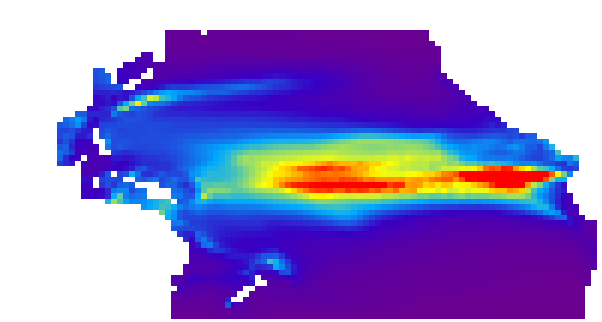
\includegraphics[width=0.4\textwidth]{annexes/figs/map_2}$ & \\
      & \vdots &  \\
      Last matrix & 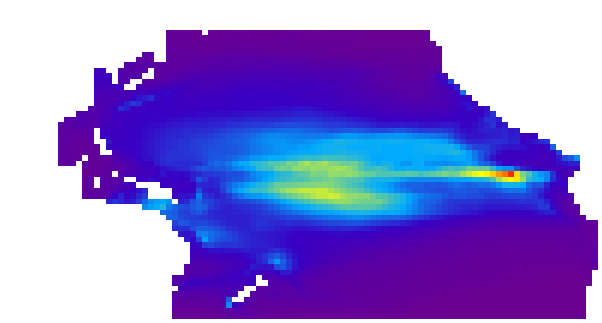
\includegraphics[width=0.4\textwidth]{annexes/figs/map_3} & \\
      \end{tabular}
    \right.$
\end{tabular}
\captionof{figure}{The order and arrangement of a two-dimensional variable in the DYM files containing {\ttfamily ZLEVEL} 2d-arrays, i.e., matrices of size NLAT$\times$NLON. Each matrix is written by rows moving in latitudinal dimension from north to south, each row includes complete longitudinal vector of values, writted from west to east. This relates to the SEAPODYM convention that the origin $(0,0)$ is placed in the north-west corner of the rectangular domain. }
\label{fig:dymvar}
\end{center} 
\end{table}

